% Chapter 4

\chapter{RJIT OSR} % Main chapter title

\label{Chapter4New} % For referencing the chapter elsewhere

%----------------------------------------------------------------------------------------

% Define some commands to keep the formatting separated from the content 
\newcommand{\keyword}[1]{\textbf{#1}}
\newcommand{\tabhead}[1]{\textbf{#1}}
\newcommand{\code}[1]{\texttt{#1}}
\newcommand{\file}[1]{\texttt{\bfseries#1}}
\newcommand{\option}[1]{\texttt{\itshape#1}}

%----------------------------------------------------------------------------------------
This chapter presents RJIT OSR, our implementation of on-stack replacement, based on the OSR Kit~\cite{OSRKit} library, that enables runtime deoptimization in R.
The first section presents an overview and introduction to our work, by describing RJIT OSR goals, the limitations encountered in OSR Kit and RJIT, our LLVM-based just-in-time compiler for R.
The second section presents RJIT OSR's implementation.
The third section presents prototypes and extensions implemented for RJIT OSR.

\section{Overview}
\subsection{Justification \& Goals}\label{justificationgoals}
            
R is a programming language and software environment for statistical computing and graphics, developed by the R Foundation for Statistical Computing~\cite{RURL}.
R is a dynamic, lazy, functional, object oriented programming language where the basic data type is the vector.
The dynamic features provided by the language include reflection over the environment, the ability to generate source code for unevaluated expressions and to treat text as code (e.g., functions \textit{parse} and \textit{eval}).
Even though R is considered functional, i.e., functions are first-class values, and arguments are deep copied and lazily evaluated, the language does not optimize recursions and, instead, encourages vectorized operations.\\

Although very flexible and widely used for statistical data analysis~\cite{RUsage}, the R programming language's implementation suffers from poor execution performance, compared to equivalent programs executed in C or Python~\cite{morandat2012evaluating}.
According to \citean{morandat2012evaluating}, on the Shootout baseline benchmarks suite~\cite{Shootout}, R is on average 501 times slower than C and 43 times slower than Python.
According to ~\cite{morandat2012evaluating}, R programs usually consume large amounts of memory, and spend an important part of the execution (e.g., on average 30\% for the Shootout benchmarks) doing memory management.
These slow downs have various causes.
For example, in R, all user data must be heap allocated and garbage collected, when languages like C allow stack allocated data.
Data boxing also impacts on R programs memory consumption.
All numeric data have to be boxed into vectors, leading to high overheads in programs containing an important amount of single numbers.
For example, in the Bioconductor corpus of programs~\cite{Bioconductor}, 36\% of vectors allocated contained only a single number~\cite{morandat2012evaluating}.
It is important to note that other R specific behaviors, such as looking up variables, matching parameters with arguments, and copy-on-write mechanisms used for call-by-value semantics have non negligible impacts on R programs performance~\cite{morandat2012evaluating}.\\

The RJIT project~\cite{Rjit} strives to improve R performance by providing an LLVM based JIT compiler for the language.
The RJIT compiler plugs into a modified version of the GNUR~\cite{RURL} interpreter and enables to JIT compile R programs into native code.
The RJIT compiler is still pretty young, only a few months old.
As a result, RJIT is currently trying to identify code behaviors that impact the execution performance, and plans to optimize code compilation to decrease their costs.
Due to R semantics, such compilation optimizations might be hard to implement.
More specifically, as explained above, R performance limitations are intrinsically linked to R semantics.
On-stack replacement therefore appeared as an interesting solution to enable aggressive and speculative optimizations, able to generate compiled code that does not respect R semantics, while preserving the overall program's correctness.
The goal of this master thesis is thus to prototype a flexible and extensible OSR mechanism for speculative optimizations in RJIT.\\

This master thesis prototypes OSR runtime deoptimization mechanisms in RJIT.
The RJIT OSR implementation relies on the OSR Kit~\cite{OSRKit} library transition mechanism.
The OSR Kit library code is available on Github~\cite{OSRKitGit}.
Instead of reimplementing the same transition mechanisms for RJIT OSR, the choice was made to modify and extend this library.
This enables to focus on the deoptimization case which, according to section \ref{WhyDeopt}, is the most challenging and interesting use case of on-stack replacement.
The OSR deoptimization further allows speculative optimizations, which enable the RJIT compiler to port static compilation optimizations to R, while preserving the correctness of the program being executed.\\

\subsection{OSR Kit Limitations}\label{osrkitlimitations}

%While very flexible, comes short on several points
    %Open OSR, not really fitting our case.
    %Continuation style is fine for optimization, but pretty bad for deopt.
        %no replacement when exits... 
        %many clones ... 
        %As we'll see later, cloning is not sufficient ...
While very flexible, the OSR Kit~\cite{OSRKit} library presents several disadvantages and exhibits costly behaviors that do not perfectly fit the deoptimization process.
This section lists the OSR Kit library's limitations with regard to OSR exits implementation.\\

The main advantage of an open OSR is to leverage profiled-guided compilation strategies to generate efficient code.
However, generating a transformation that removes optimizations is hard and does not play well with the OSR Kit instrumentation.
Such a transformation needs to take into account other optimizations that might have been performed on the code after the invalidated one, i.e., deoptimizing requires to keep track of which transformations performed on the code depend on the invalidated optimization, and undo them.
At the OSR point, the framework relies on a StateMap that matches values in the from and the continuation functions.
That implies that, in order to generate the continuation function on the fly for the deoptimization case, one is required to 1) be able to reverse an optimization, that might have interfered with other transformations, and 2) to generate a correct StateMap to give as input to the OSR Kit machinery.
Both of these requirements are hard to satisfy.
Finally, the deoptimization case is used to preserve correctness in the program and must be conservative. 
Performance is a soft issue, and hence leveraging profiled-guided compilation strategies is not primordial.\\

Once an OSR exit is taken, it is more likely to be fired in subsequent executions.
For example, in the case of call site inlining, the OSR exit is fired when the inlined function is redefined.
Once the function has been redefined, the OSR exit is expected to be triggered at every execution.
As a result, if the OSR exit is an open OSR point, the framework will have to perform expensive operations to generate the correct continuation function at every execution of the invalidated function.
In the light of these observations, we can conclude that the open OSR design does not fit well the deoptimization case.\\

The resolved OSR corresponds to our requirements for deoptimization.
The optimized version is obtained by applying a transformation on a base function.
Since OSR points cannot be tampered with, the mapping between the OSR exit and the base function is guaranteed to be preserved, regardless of the subsequent (valid) optimizations performed on the optimized function.
Another way to see this is that the OSR exit is a call to the continuation function, which takes as arguments all the values needed at the landing site to reconstruct the computation state and continue the execution.
As long as the OSR exit call is preserved, and its arguments valid, the continuation function should be able to execute properly.
For the overall execution to be correct, additional constraints, such as preventing instructions with side-effects from crossing OSR points, are however still required.
In the light of these observations, it makes sense to instrument the base function to generate a continuation function for the exit.\\

The OSR Kit way of generating the continuation function is expensive.
In the deoptimization case, inserting a resolved OSR exit requires to 1) clone the base function in order to obtain two copies: one is kept as is, the other will be optimized, 2) generate the continuation function. 
Since the continuation function might have a different signature than the base function, the framework has to clone the body of the base function that will be instrumented with the \codekey{OSR\char`_ENTRY} block.
Generating two clones of the base function, in order to insert a resolved OSR exit, might be very expensive for big functions.\\

Finally, as it was the case for the open OSR, the resolved OSR does not take into account the fact that an OSR exit might be triggered at every call, once it has been fired a first time.
Although less expensive than the open OSR, a resolved OSR exit that fires at every execution adds the costs of evaluating the OSR condition, and a function call and return, compared to the base unoptimized function.
The OSR Kit framework does not provide the mechanisms required to avoid this extra cost.\\

\subsection{The RJIT Compiler}
\subsubsection{General}

%General information
The RJIT project is an LLVM based JIT Compiler for the R programming language.
It relies on GNUR~\cite{RURL}, an interpreter for R. 
GNUR provides an abstract syntax tree interpreter, a bytecode compiler and a bytecode interpreter for R.
The RJIT compiler takes as input a symbolic expression (SEXP), i.e., a special C structure generated by GNUR while parsing R programs.
A SEXP contains the AST representation of an R construct.
A SEXP has a type, and can be seen as a lisp-like cons cell, composed of two pointers, CAR and CDR.
A SEXP has many other elements, that we do not detail here.
Depending on its type, each SEXP element corresponds to a specific attribute (see examples for closures and functions below). 
The GNUR interpreter has been instrumented to call the JIT compiler before evaluating a non-compiled SEXP. 
RJIT generates native code, using the LLVM framework, that corresponds to the R abstract syntax tree.
The native code is then wrapped into the appropriate SEXP constructs, and returned to the GNUR interpreter.
Afterwards, the GNUR interpreter executes the native code.\\ 

\begin{figure}[h]
    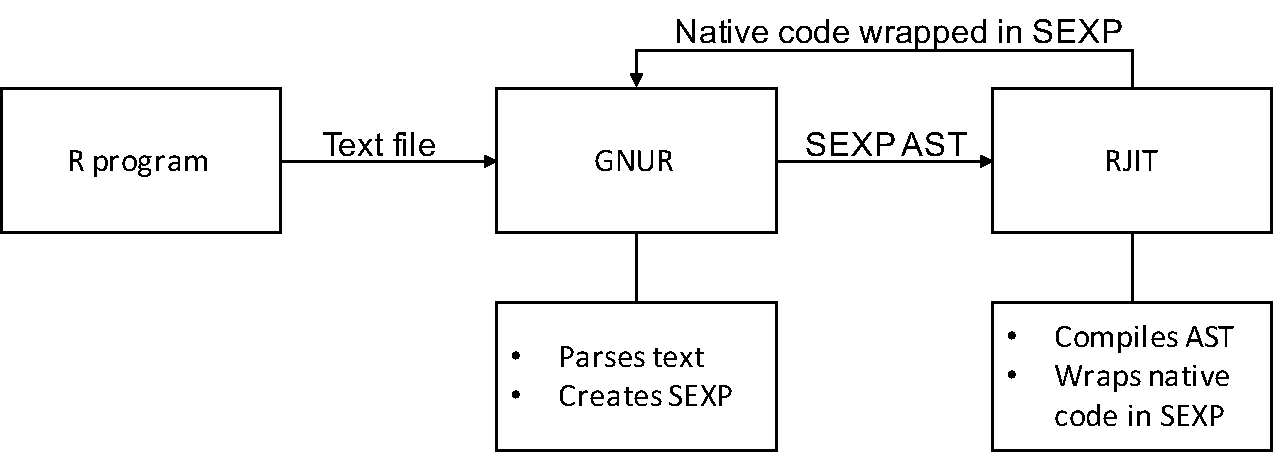
\includegraphics[scale=0.5]{Figures/RJITFlow}
    \caption{RJIT compilation flow.}
\end{figure}

\subsubsection{The compilation flow}
RJIT walks the SEXP AST and generates the corresponding LLVM IR.
Since R is a dynamic language, most R constructs need to be simulated by LLVM calls to special functions, called R intrinsics.
Intrinsic functions provide basic functionalities, such as resolving a closure from a symbol and the current environment, getting a value associated with a symbol, setting a local variable, creating a promise, or performing generic arithmetic operations.
Figure \ref{fig:exampleirforr} provides R code performing some of these standard operations (lines 1-5), and the equivalent, simplified, LLVM IR, with the corresponding intrinsic calls.\\

\begin{figure}[h]
\includecode{Code/RAndLLVM.cpp}
\caption{Example of LLVM IR for basic R code.}
\label{fig:exampleirforr}
\end{figure}

R resolves the target of a function call at runtime, when the call is executed.
In order to simulate this behavior, the RJIT compiler needs to rely on a special instrumentation to compile calls to functions, especially the ones to functions that are not yet defined.
To that end, the JIT compiler replaces function calls with inlined cached stubs (i.e., ic stubs).
An ic stub (e.g., line 18 in Figure \ref{fig:exampleirforr}) takes as parameters the function call's arguments, the caller's constant pool, a pointer to the callee extracted from the environment, the caller's environment and a pointer to the caller.
The ic stub, when executed, triggers the compilation of a wrapper function, call it the ic callee, that caches the resolved callee.
This wrapper function tests that the callee pointer that it gets as argument points to the same function as the one used during its own compilation.
If that is the case, it performs the call to the callee, and propagates the value returned after the call.
If the callee pointer references another function, it performs an ic stub call.
Once the ic callee function is compiled, the ic stub replaces itself in the caller with a call to the ic callee.
In order to do so, the ic stub relies on LLVM intrinsics called stackmaps\cite{llvmStackMap} and patchpoints\cite{llvmPatchpoints}, and on the caller's pointer it received as argument.\\

The compilation flow can be reduced to the following steps:
\begin{enumerate}
    \item The function's AST is extracted from the SEXP.
    \item The JIT compiler traverses the AST and produces the corresponding LLVM IR.
        \begin{itemize}
        \item Calls to non-intrinsic functions are translated into ic stubs.
        \item Safepoint and patchpoint ids are set at every call instruction as LLVM attributes\cite{llvmAttribute}.
        \end{itemize}
    \item When the \textit{jitAll} function is called on the compiler instance, every call instruction in every function in the module is visited.\label{jitAll}
        \begin{itemize}
        \item Safepoints are inserted at every call and used by the garbage collector during the execution.
        \item Patchpoints\cite{llvmPatchpoints} are inserted at ic stubs.
        \end{itemize}
    \item The native code corresponding to each function is generated and inserted into the corresponding SEXPs.
\end{enumerate}

The output of the compiler at step \ref{jitAll} is a blotted piece of LLVM IR from which R semantics are hard to extract.
Figure \ref{fig:RSimpleFunction} defines a very simple R function.
Figure \ref{fig:noninstrumentedir} provides the non-instrumented RJIT LLVM IR.
Figure \ref{fig:instrumentedir} provides the RJIT LLVM IR instrumented with safepoints.\\

\begin{figure}[h]
    \includecode{Code/Rfunction.c}
        \caption{R simple function.}
        \label{fig:RSimpleFunction}
\end{figure}

\begin{figure}[h]
    \includecode{Code/UninstrumentedIR.c}
    \caption{Non-instrumented RJIT LLVM IR.}
    \label{fig:noninstrumentedir}
\end{figure}

\clearpage
\begin{landscape}
\begin{figure}[h]
    \includecode{Code/InstrumentedIR.c}
    \caption{Instrumented RJIT LLVM IR.}
\label{fig:instrumentedir}
\end{figure}
\end{landscape}
\clearpage


\subsubsection{The function's SEXP}
In GNUR and RJIT, a function is represented by a special SEXP. 
This SEXP has a \codekey{NATIVESXP} type when the function is compiled by the RJIT compiler, and a \codekey{LANGSXP}, i.e., a language construct, when it is not.
In the case of a compiled function, the \codekey{CAR} element contains a pointer to the native code of the function.
The \codekey{CDR} element, in both cases, contains the constant pool associated to the function, i.e., the list of symbols defined inside the function.
For a compiled function, the \codekey{TAG} element of the SEXP contains the function's LLVM IR.\\

When the GNUR interpreter evaluates a function SEXP, it checks its type. 
If the function is compiled, it performs the call to the native code. 
If not, it calls the RJIT compiler, and executes the resulting native code.\\

In RJIT, the LLVM IR for a function always has a signature of type $T$:
$$T: (\text{SEXP}, \text{SEXP}, i32) \rightarrow \text{SEXP}.$$
where the first SEXP element is a pointer to the constant pool associated with the function, and the second SEXP a pointer to the environment.
As shown in Figure \ref{fig:exampleirforr}, the constant pool (CP) is used to access variable symbols. 
For example, line 11 corresponds to a call to the \codekey{genericGetVar} intrinsic, that enables to retrieve a local variable's value from the environment.
The symbol corresponding to the variable is extracted from the CP, at index 2, and used along side the environment (i.e., \codekey{rho}), to access the corresponding value.
In general, the environment is used to access variable values as well as function definitions (e.g., line 15).\\


\subsubsection{The closure's SEXP}
In R, a closure contains a function and the environment associated to it.
A closure SEXP has type \codekey{CLOSXP}.
The \codekey{BODY} element of a SEXP closure is a function SEXP.
The \codekey{TAG} of a SEXP closure is an environment SEXP, of type \codekey{ENVSXP}.
The environment is made of cons cells, and is essential to the execution of a function.
Local variables and function argument values are set inside the environment.
A closure also contains the formals, i.e., the arguments symbols of the function.
The \codekey{getFunction} intrinsic, that enables to resolve a function, returns a closure.\\


\section{OSR Handler}
This section presents the OSR Handler, a special singleton implemented in RJIT that strives to enable efficient OSR deoptimizations. 
The OSR Handler has two main goals: 1) to mitigate the limitations of the OSR Kit~\cite{OSRKit} library exposed in \ref{osrkitlimitations}, 2) to adapt the OSR Kit library to the RJIT compiler.\\

This section proceeds as follow: first, it exposes the additional challenges that are inherent to the use of the OSR Kit library in RJIT.
Then, it presents the OSR Handler implementation, and the solutions adopted for each problem encountered while enabling OSR deoptimization in RJIT.\\
 
\subsection{Additional Challenges in RJIT}\label{additionalchallenges}

The RJIT LLVM IR uncovers additional challenges in the use of OSR Kit~\cite{OSRKit} for the deoptimization case.
RJIT LLVM IR specificities, such as the instrumentation for the garbage collector and the ic stub calls, require specially care when used along side the OSR library.\\

In order to perform transformations based on R semantics, a fresh non-instrumented (i.e., without the safepoint and patchpoint machinery) version of the LLVM IR is needed.
The non-instrumented IR corresponds to the compiler's output, before calling the \codekey{jitAll} function.
For functions that were never compiled, invoking the compiler and extracting the non-instrumented IR seems like a reasonable solution.
However, for functions that were fully compiled previously, i.e., functions that have an instrumented LLVM IR, re-parsing ASTs in order to obtain a non-instrumented IR is not a satisfactory solution.
We therefore have to find a way to avoid re-generating functions IR unnecessarily.\\

Simply cloning the LLVM IR is not enough in RJIT.
In order to fully compile and execute a clone, its LLVM attributes need to be set at each of its call instructions to allow safepoint instrumentation.
This is mandatory and, if not done properly, leads to failures during the execution.
Another problem with clones arises from the targets of function calls.
In LLVM, a callee has to be an LLVM function declared in the same module.
Therefore, compiling a clone of a function compiled in a different module requires to ensure that every callee is defined in the current compilation module.
One last thing to take care of are the ic stubs calls.
An ic stub takes as argument a pointer to its caller.
When a function containing ic stubs is cloned, the caller pointer arguments point to the original function.
This needs to be fixed if the clone is to be fully compiled and executed.
Section \ref{osrkitlimitations} states that one drawback in the OSR Kit implementation comes from the number of clones that have to be generated to insert a resolved OSR point.
In RJIT, the cost of fixing the LLVM IR, as explained in this paragraph, has to be added to the cost of cloning.\\

OSR Kit continuation functions are not compatible with ic stubs.
The ic stubs expect to receive pointers to their callers as argument.
In RJIT, every function is supposed to have the following type signature:
$$T: (\text{SEXP}, \text{SEXP}, i32) \rightarrow \text{SEXP}.$$
According to Section \ref{describeOSRKit}, the OSR Kit\cite{OSRKit} library modifies the continuation function's signature in order to pass all the live values during an OSR transition.
As a result, the continuation function might not be of type $T$.
Enabling any type in the ic stub is not a viable solution, i.e., it requires too much work and goes against the type policies enforced by the RJIT framework. 
We therefore have to come up with an alternative solution.\\

The next sections present the solutions implemented in RJIT to mitigate the OSR Kit limitations in the deoptimization case, while answering the above challenges particular to the RJIT framework.\\

\subsection{Reducing the Number of Compilations}\label{section:reducecompilations}

Transformations that act on R semantics have to be performed on a non-instrumented LLVM IR.
As explained before, obtaining such IR might be harder than expected. 
There are three cases to distinguish:
\begin{enumerate}
    \item The function was never compiled before.\label{toCompile}
    \item The function was compiled, but not instrumented.\label{best} 
    \item The function was compiled and instrumented.\label{worst}
\end{enumerate}

For case \ref{toCompile}, the only option is to compile the function, and extract the generated IR before the final instrumentation.
Case \ref{best} is the best scenario.
The LLVM IR can simply be extracted from the SEXP function, cloned, and used for the transformations.
This case happens when the function was compiled during the current compilation unit, i.e., the function is part of the current module and was generated using the current instance of the compiler, on which the \codekey{jitAll} function was not called yet.
Case \ref{worst} is the worst scenario.
The non-instrumented LLVM IR no longer exists.
The naive solution is to recompile the function from scratch, i.e., re-parse the corresponding AST and emit the corresponding non-instrumented LLVM IR, which seems very expensive.\\

The OSR Handler enables to record non-instrumented IRs that it encounters.
Non-instrumented IRs are registered in the \codekey{baseVersions} map, a map from a SEXP closure to a \codekey{NATIVESXP} function SEXP.
This singleton provides a special function, called \codekey{getFreshIR}, that takes as parameter a SEXP closure and a compiler instance, and returns a function SEXP (see signature Figure \ref{fig:getfreshir}).
The OSR Handler extracts the function from the closure, and checks its type.
Depending on the type of the function and the content of the \codekey{baseVersions} map, it selects the less costly solution to get the non-instrumented IR.\\

\begin{figure}[h]
\includecode{Code/getFreshIR.h}
\caption{The getFreshIR prototype.}
\label{fig:getfreshir}
\end{figure}

The OSR Handler \codekey{getFreshIR} function compiles and registers non-\codekey{NATIVESXP} functions (case \ref{toCompile}).
The OSR Handler invokes the compiler on the function, and creates two clones of the resulting non-instrumented IR.
Both clones are not part of the current compilation module, i.e., their IRs are not instrumented when the \codekey{jitAll} function is called.
One clone is wrapped inside a copy of the function SEXP and stored in the \codekey{baseVersions} map.
The other clone is also wrapped inside a copy of the function SEXP and returned to the user.\\

Calling \codekey{getFreshIR} on a function that was not previously compiled can be viewed as an ahead of time (AOT) compilation strategy.
RJIT is a JIT compiler, i.e., functions are compiled just before being executed.
Using the \codekey{getFreshIR} can force the function's compilation to happen at anytime.
As a small optimization, the OSR Handler sets the result of the compilation inside the corresponding closure.
By doing so, we ensure that a subsequent call to this function will already benefit from the compiled version, and will not trigger a useless call to the JIT.\\

The \codekey{getFreshIR} strives to avoid having to re-generate LLVM IR for \codekey{NATIVESXP}s.
When the closure passed as argument to the \codekey{getFreshIR} call has an entry in the base version map, a clone of the stored function SEXP is returned.
Cloning the function SEXP requires to clone the LLVM IR, and insert it in a new function SEXP with the same constant pool.
When the closure passed as argument does not have an entry in the base version map, the OSR Handler must determine if the IR is instrumented or not.
RJIT creates one module per compiler instance, and performs the \codekey{jitAll} call just before returning to the interpreter.
As a result, if an LLVM IR's module is the same as the current compiler's module, the LLVM IR is not instrumented.
In this case, the \codekey{getFreshIR} function creates an entry for this closure in the \codekey{baseVersions} map and returns the proper clone to the user, as explained before.
For an LLVM IR with a different module, that does not have an entry in the base version map, the OSR Handler has no other choice than to re-parse the ASTs and generate the non-instrumented LLVM IR.
In this case, it also creates a proper entry in the \codekey{baseVersions} map and returns a copy to the user.
This situation can be avoided by making sure that for every function compiled, a proper entry is registered in the OSR Handler's \codekey{baseVersions} map.\\

\begin{figure}[h]
\includecode{Code/baseVersion.h}
\caption{The base version map.}
\label{fig:baseversionmap}
\end{figure}

The non-instrumented IR obtained through the \codekey{getFreshIR} function corresponds to the original AST of the function, i.e., no transformation has been applied on this IR. 
In other words, all the transformations performed while compiling the function the first time are not reflected on the stored IR. 
This allows to keep different optimization passes independent.
In some cases, that solution implies that we have to apply the same transformation on the same function several times.
For example, consider a function $A$ that calls $B$ several times.
An inliner would inline every call sites in $A$.
The inliner could further decide to inline all the calls inside $B$'s body.
In that case, if the inliner relies on the OSR Handler to get $B$'s IR, it will have to run on each separate clone to inline the call sites they contain, therefore performing the same transformations multiple times.
On the other hand, if the inliner's transformations depend on the location of the call to $B$, it is guaranteed to obtain fresh and independent IRs via the OSR Handler.\\

\begin{figure}[h]
\includecode{Code/utilities.h}
\caption{Utility functions.}
\label{fig:utilityfunctions}
\end{figure}

A cloned function that needs to be fully compiled has to be fixed.
As explained in Section \ref{additionalchallenges}, the IR of a cloned function has incorrect attributes instrumentation, incorrect arguments to its ic stub calls, and might have missing targets in its call instructions, i.e., the callee has not been declared in the module.
A cloned function also needs to be added to the compilation module in order to be fully compiled.
The OSR Handler provides utility functions to help the user fix the LLVM IR of cloned functions in RJIT. 
The \codekey{resetSafepoints} function takes care of adding the proper safepoints and patchpoints to the IR, as well as fixing the ic stubs arguments.
It further verifies that every callee in call instructions has been declared in the module. 
If that is not the case, it adds the proper function definition to the module.
The OSR Handler provides another function, \codekey{addSexpToModule}, that enables to add a function to the current compilation module.
Finally, the compilation engine requires to register an explicit mapping between an LLVM IR and a SEXP to properly link the generated native code in the function SEXP.
The \codekey{addRelocation} function enables to register a mapping between a cloned SEXP and the cloned LLVM function it contains.
These utilities functions are implemented so that each of them provides a single, fully contained functionality. 
It enables the user to have a fine-grained control over the LLVM IR clones, and only perform the desired operations.\\

The SEXP entries in the \codekey{baseVersions} map are subjected to garbage collection.
When a garbage collection is triggered, the R garbage collector might need to collect values inside the map.
For the moment, the OSR Handler deletes all the entries contained in the map whenever a garbage collection happens.
Preventing the collection of these items would introduce an important memory leak, since any non-live function would still have an entry in the map.
Completely deleting the entries is, however, a drastic solution.
A better solution would be to delete only items that correspond to closures that are no longer live, and protect the other entries.
This solution requires a tighter interaction with the garbage collector and was not implemented. 
We however devise an alternative solution in section \ref{section:futurework}.\\

\subsection{Simplifying the OSR Exit Insertions}

Section \ref{osrkitlimitations} explains our choice to use resolved OSR from the OSR Kit\cite{OSRKit} library.
The resolved OSR API is provided in Section \ref{describeOSRKit}.\\

RJIT imposes additional constraints on the OSR exits. 
The continuation instruction needs to be the exact match of the from instruction.
In other words, considering the \codekey{insertResolvedOSR}, the \codekey{lPad} argument is the instruction in the continuation function that corresponds to the \codekey{src} argument in the from function.
The OSR Kit library provides some flexibility in the choice of these two instructions. 
This flexibility is not required in RJIT, and is removed to ensure the implementation's correctness.\\

The OSR Handler provides a special cloning function, called \codekey{getToInstrument}, that clones an LLVM function, adds it to the same module as the original function, fixes its IR, and automatically registers a StateMap between the original and the cloned function in its \codekey{statemaps}, a map from a pair of LLVM function pointers to a StateMap (see Figure \ref{fig:statemaps}).\\

\begin{figure}[h]
\includecode{Code/statemaps.h}
\caption{The statemaps.}
\label{fig:statemaps}
\end{figure}

The \textit{toInstrument} clone is the argument passed as the continuation function to the \codekey{insertResolvedOSR} call.
As explained in Section \ref{osrkitlimitations}, the OSR Kit library will clone the \textit{toInstrument} function to generate the continuation.
It relies on a StateMap that is passed as argument to the function call. 
Thanks to the OSR Handler's \codekey{statemaps}, this argument can be omitted and automatically retrieved.\\

The \textit{toInstrument} function is added to the module, and will therefore be fully compiled upon the \codekey{jitAll} call.
As explained in Section \ref{additionalchallenges}, the continuation function's ic stub calls cannot use the continuation function's pointer as argument for the caller. 
The toInstrument function's address is used instead, which in turns requires the toInstrument function to be part of the module and go through the entire compilation.
The toInstrument function has another important role detailed in Section \ref{improvingexits}.\\

The OSR Handler provides a function, called \codekey{insertOSRExit}, that exhibits the simplified interface described in this section to insert OSR exits.
The function's prototype is provided in Figure \ref{fig:insertoserexit}.
Section \ref{improvingexits} describes in details the role of the last argument.\\

\begin{figure}[h]
\includecode{Code/insertOSRExit.h}
\caption{The \codekey{insertOSRExit} prototype.}
\label{fig:insertoserexit}
\end{figure}

\subsection{Improving the Exits}\label{improvingexits}
%OSR kit not well suited for osr exits. 
%The call stub when executed will go replace itself in the toInstrument function, not in the stub.
%Hence compensation 

The continuation function mechanism does not fit the OSR exits well.
As explained in Section \ref{osrkitlimitations}, once an OSR exit is fired, it is likely to be fired in subsequent calls.
Triggering an OSR exit has a cost that might not be negligible.
The OSR Kit~\cite{OSRKit} library does not provide any mechanism to improve that special case.
Moreover, section \ref{additionalchallenges} explains that continuation functions do not have valid signatures for ic stubs, which requires to come up with a special hack to make them work properly.\\

The OSR Handler, via the \codekey{insertOSRExit} method, enables to add a special compensation code at the beginning of the \codekey{OSR\char`_ENTRY} block in the continuation function, to answer these limitations.
The compensation code can be any valid vector of LLVM instructions.
This can be used to avoid triggering the OSR exit repeatedly once it has been fired a first time.
For example, the compensation vector can contain a special call to a C++ function, that takes as argument a unique identifier for the continuation function. 
The C++ function then uses this identifier to retrieve the corresponding toInstrument function.
The toInstrument function is a valid, fully compiled version of the original function, that does not contain the invalidated optimization.
The C++ function then replaces the incorrect optimized function by the toInstrument function in the closure.
As a result, all subsequent calls to the closure will execute a correct version of the function.
This enables to avoid the cost of triggering an exit upon every call.\\

The compensation code in the OSR Handler does not rely on the OSR Kit compensation code mechanism.
The OSR Kit compensation code is used to fix the execution state, is associated to values transferred from one version to another, and is not meant to access the execution environment.
Since it pertains to a different goal, we decided to implement our own solution.
The instructions that enable to replace the function's version in the closure are left to the user. 
This provides some flexibility on how to decide whether or not to replace the current function.\\

Replacing the invalidated optimized version by the \textit{toInstrument} function presents several advantages.
First, since the \textit{toInstrument} was used to generate the continuation function, we know that it is correct and does not contain the invalidated transformations.
Second, when the continuation function's ic stubs are executed, the RJIT framework generates inlined cached version of the target function, and is supposed to replace the ic stubs by a call to this inlined cached functions.
For that purpose, it uses the ic stub argument that points to its caller.
This argument, in the continuation function, points to the \textit{toInstrument} function.
As a result, when the continuation function's ic stubs are executed, the ic stubs in the toInstrument function are replaced by inlined cached functions, which are supposed to be faster.
This ensures that taking an OSR exit will have as little impact on the overall execution time as possible.
Furthermore, this mechanism ensures that executing a function twice, while experiencing an OSR exit in the first execution, will still have good performances compared to executing the non-optimized version the same number of times.\\

\subsection{Walkthrough a Simple Example}
In this section, we provide a full example of a possible use of the OSR Handler's mechanisms.
It describes which functions are called, and how every element is used.
This example enables to show how the OSR Handler abstracts away all the different challenges that we described before, and enables to focus on the transformations performed on the input function.\\

Assume a transformation process \codekey{TransP}, that speculatively inlines function calls inside the input function. 
\codekey{TransP} receives as input the closure to optimize, and returns a closure containing the optimized version of the code.
Every function call inlined has a special OSR exit instrumentation to handle runtime redefinition of the inlined functions.\\

\codekey{TransP} gets the LLVM IR corresponding to the input function by calling the OSR Handler \codekey{getFreshIR} function.
Call this copy the \textit{working copy}.
It then lists all the function calls performed inside the IR.
For each function call, sequentially, it gets a \textit{toInstrument} copy of the working copy by calling the OSR Handler clone function.
Each toInstrument is wrapped into its own SEXP, added to the module, has its IR corrected by the \codekey{reseSafepoints} function, and is added to the relocations for the final native code to SEXP mapping.
\textit{TransP} resolves the callee, and gets its LLVM IR via the OSR Handler \codekey{getFreshIR}.
It then inlines the call in its working copy and calls the OSR Handler \codekey{insertOSRExit} function.
It then calls the \codekey{resetSafepoints} on the working copy to fix the IR, and returns its enclosing closure.
The working copy contains all the OSR exits needed for correctness, all the continuation functions, and their corresponding \textit{toInstrument} versions are generated and part of the current module.
Thanks to RJIT OSR, \codekey{TransP} was able to locally break R semantics by inlining function calls, while preserving the overall correctness of the program.\\


\section{Other prototypes \& Future work}\label{section:futurework}
This section describes solutions, design ideas, that were partially implemented but not fully explored during this master thesis.
RJIT being a young project, it lacks some supporting tools, e.g., a profiler or a profiled-base recompilation mechanism, that could uncover new possibilities for the OSR implementation.
In the future, the development of the RJIT framework should enable to provide new incentives to implement more complex OSR-based speculative optimizations, or extend the OSR mechanisms.\\

\subsection{Transitive StateMaps}
%Trying to improve the field of possibilities
    %Chain of statemaps, can find what is in common in both of them
    %Why interesting? Will be able, if provides interface, to enlarge the scope of intermixing optimizations 
For the moment, in RJIT, the continuation function for an OSR exit is an instrumented version of the function that was used to generate the optimized version.
This is a requirement that results from the use, in OSR Kit~\cite{OSRKit}, of StateMaps to insert the OSR instrumentation.
The from and the continuation functions need to have a StateMap that records one-to-one mappings between their instructions.
In some cases, however, one might want to provide a different continuation function.
OSR Kit does not forbid this use of the library, but does not provide tools to make it easier.\\  

Consider the following chain of speculative optimizations performed on a base function $A$: 
$$A \xrightarrow[]{1} B \xrightarrow[]{2} C \xrightarrow[]{3} D \xrightarrow[]{4} E \xrightarrow[]{5} F \rightarrow ...$$
Each letter corresponds to a new version of the function. 
Each version is obtain by performing a speculative optimization of the previous version.
If an assumption fails, the continuation function will be an instrumented version of the base version on which the speculative optimization was performed.
For example, if the current version is $F$, and the OSR exit that corresponds to arrow 3 is taken, 
the function will exit to a continuation function that corresponds to version $C$.
One might want, instead, to OSR exit to $A$, or to generate on the fly a new continuation function that underwent all the transformations, except number 3. 
This might not always be possible, and requires to understand all the interactions between the different optimizations.
However, if all the transformation are independent, i.e., if none of them impacts on the others, this should be feasible.
We should be able to find a corresponding continuation instruction in any other version.\\

As a first step towards a more complex mapping between the from and the continuation function, we implemented a transitive StateMap constructor.
Suppose two fully generated StateMaps, $S_1$ and $S_2$, such that $S_1$ is a mapping between $A$ and $B$, and $S_2$ a mapping between $A$ and $C$.
Our transitive constructor enables to generate a new StateMap, $S_3$, that maps $B$ and $C$.\\

The transitive constructor can be extended to create StateMaps between different functions, generated by applying an arbitrary number of transformations on the same base function.
Consider the above chain of transformations.
The transitive StateMap constructor can be used to generate a transitive map between every pair of versions in the chain.
The resulting StateMap might not be complete, but it ensures that every instruction that is present in the base version $A$ and both versions that we want to map, e.g., $C$ and $F$, will be present in the resulting StateMap.\\

If we further extend the framework to automatically update the StateMap while modifying an LLVM IR, we might even be able to uncover new possible mappings between different versions, and lift the restriction on the transitive StateMaps, i.e., we could generate mappings between instructions, even if they do not appear in $A$ and in both versions $C$ and $F$.
This solution would be similar to the VARMAP in the Jikes RVM OSR implementation~\cite{soman2006efficient}.
According to a discussion we had with the OSR Kit designers, \citean{OSRKit} are working on a similar idea on the OSR Kit build compensation branch~\cite{OSRKitGit}.
The idea is to provide basic LLVM transformation functions, e.g, addInstruction, removeInstruction etc., that automatically update the StateMap.\\

\subsection{Unguarded OSR Points \& Lazy Deoptimization}

The OSR Kit~\cite{OSRKit} library only provides guarded OSR points.
As explained in section \ref{section:osrpoints}, unguarded OSR points correspond to portions of the code that can be overwritten, at runtime, based on external events detected by the runtime framework.
In certain cases, unguarded OSR points enable to decrease the overhead introduced by the OSR mechanisms. 
For example, consider the unoptimized function in Figure \ref{fig:lazydeoptnorm}. 
In \codekey{f}, the variable \codekey{x} is deemed constant. 
The compiler would therefore like to speculatively replace the return instruction by the value of \codekey{x}, hence avoiding the cost of an environment lookup (Figure \ref{fig:lazydeoptopt}).
A guarded OSR exit does not allow any performance gain in that case.
In fact, the guard, i.e. the OSR condition, must check that \codekey{x} is equal to \codekey{3}, and hence cancels any benefit obtained from the constant propagation optimization.
With an unguarded OSR point, however, the execution environment (here GNUR), is instrumented to detect reassignments to \codekey{x}.
Assuming there are more reads then writes, and that the value for \codekey{x} is rarely modified, we can expect the unguarded point to have a better runtime performance than a guarded one.\\

\begin{figure}[h]
    \centering
    \begin{subfigure}{.49\textwidth}
        \includecode{Code/lazyDeoptNorm.r}
        \caption{Unoptimized function.}
        \label{fig:lazydeoptnorm}
    \end{subfigure}
    \centering
    \begin{subfigure}{.49\textwidth}
        \includecode{Code/lazyDeoptOpt.r}
        \caption{Optimized Function.}
        \label{fig:lazydeoptopt}   
    \end{subfigure}
    \caption{Use case for unguarded OSR points.}
    \label{fig:unguardedosrpointexample}
\end{figure}

In RJIT OSR, we were able to construct a prototype for unguarded OSR exits and lazy deoptimization.
The base assumption is that any function call might invalidate a speculative optimization.
Each call instruction that might invalidate an assumption is therefore instrumented with a patchpoint~\cite{llvmPatchpoints} that enables to insert, at runtime, a call to the continuation function, whenever a speculative optimization is invalidated.
We were able to re-use parts of the OSR Kit library to generate the continuation function and the OSR exit call itself.
Consider the example in Figure \ref{fig:unguardedosrpointexample}.
The function \codekey{g} is unknown and might reassign \codekey{x} to a new value.
GNUR is instrumented to detect reassignments to symbols used during a speculative optimization.
It therefore detects \codekey{x} reassignements, and patches the reserved bytes following the call to \codekey{g} with a call to the OSR exit.
When \codekey{g} returns to the invalidated \codekey{f}, the call to the continuation function is executed, hence triggering a lazy deoptimization of \codekey{f}.\\

This prototype was not inserted in the final version of the OSR Handler.
Unguarded OSR points require to instrument the runtime environment, here GNUR, to collect feedback on the current execution and detect assumptions failures.
Depending on the speculative assumptions performed, different watchpoints need to be inserted inside GNUR.
As explained previously, for the moment, RJIT does not perform any adaptive optimization. 
We therefore decided to avoid instrumenting GNUR before knowing which kinds of events need to be monitored.\\

\subsection{On-the-fly Compilation}

Generating the OSR exit continuation on the fly is hard in general. 
Section \ref{osrkitlimitations} details the challenges that this technique presents.
One option to simulate this behavior in RJIT is to save the LLVM IR of the base function in the OSR Handler, and remove it from the compilation unit.
In other words, we generate and save the IR, but we do not complete its compilation.
An open OSR is inserted in the optimized version. 
The $f_{stub}$ function is then responsible for identifying the correct continuation instruction inside the saved base IR, and completing its compilation using profiled guided techniques.\\

On-the-fly compilation of continuation functions requires to guarantee that a transitive StateMap can be generated between the from function, and the newly generated function.
RJIT is not mature enough to make this solution worth exploring.
First, there is no profiler, and hence, no profile-guided transformation. 
Second, the kind of transformations that RJIT would like to perform are not yet known. 
It is too early in the implementation process to identify which optimizations might improve the execution of the function.
As a result, we did not put efforts in the implementation of this solution.\\

\subsection{A Better Integration}\label{section:cleanerIR}

The OSR Handler is a prototype, a proof of concept, to experiment with OSR transitions in RJIT. 
As such, the choice was made, at the beginning of the implementation, to encapsulate everything related to the OSR deoptimization mechanism, e.g., the OSR Handler, the OSR inliner (see chapter \ref{Chapter5}), in their own classes.
In other words, everything added to RJIT was kept as independent to the main RJIT elements as possible.
This had the double benefit of 1) enforcing clear and stable interfaces that integrate well in the compilation flow, and 2) enabled to merge the master branch updates into the OSR branch easily.
Since the RJIT project is under active development, the second point was essential.
On the other hand, the OSR mechanisms could be greatly simplified, and made cleaner, if properly integrated inside the RJIT framework.\\

The OSR Handler, and more specifically the base versions map, could be, in the future, replaced by a careful instrumentation of the function's SEXP. 
For the moment, the \codekey{TAG} attribute of a compiled function's SEXP contains the LLVM IR used to generate the native function.
If the function went through the entire compilation flow, the LLVM IR is instrumented. 
In RJIT, this \codekey{TAG} LLVM IR is mostly used for debugging purposes.
In the future, a non-instrumented snapshot of the function's module could be stored instead.
When a transformation needs to be performed on an already compiled function, the snapshot can be loaded inside the current compilation module, and the non-instrumented LLVM IR of the function extracted from it.
This has the double benefit of easily providing an LLVM IR to work on, while removing any need to fix call instruction targets in the IR (see section \ref{additionalchallenges} for more details on this matter).
This also enables a better integration with R garbage collector. 
LLVM IRs can be collected at the same time as their enclosing closures, without requiring any additional mechanism.\\

For the moment, many parts of the implementation rely on the fact that a function's SEXP \codekey{TAG} contains the LLVM IR of the native code. 
As a result, this would not be a trivial change and needs the approval of the entire team.
However, after talking to the main developers, the decision was made to make this change happen in the future.\\